%%%%% Brief Journal Paper version %%%%%
\documentclass[letterpaper, 11 pt, journal, twoside]{IEEEtran}

\usepackage{mathrsfs}
\usepackage{amssymb}
\usepackage{amsmath}
\usepackage{epsfig}
\usepackage{graphicx}
\usepackage{color}
\usepackage{cite}
\usepackage{url}

%%%% Selective part from steve.lib
\newcommand{\rank}{{\rm rank\;}}
\newcommand{\image}{{\rm Im\;}}
\newcommand{\stack}{{\rm stack\;}}
\newcommand{\Span}{{\rm span\;}}
\newcommand{\diag}{{\rm diag\;}}
\newcommand{\col}{{\rm col\;}}
\newcommand{\cp}{{\rm cp\;}}
\newcommand{\R}{\mathbb{R}}
\newtheorem{theorem}{Theorem}
\newtheorem{problem}{Problem}
\newtheorem{lemma}{Lemma}
\newtheorem{remark}{Remark}
\newtheorem{proposition}{Proposition}
\newtheorem{corollary}{Corollary}
\newtheorem{property}{Property}
\newtheorem{conjecture}{Conjecture}
\newtheorem{assumption}{Assumption}
\newtheorem{exercise}{Exercise}
\newtheorem{example}{Example}
\def\n{{\bf n}}
\def\m{{\bf m}}
\def\r{{\bf r}}
\def\c{{\bf c}}
\def\scr#1{{\mathcal #1}}
\def\rep#1{(\ref{#1})}
\def\eq#1{\begin{equation}#1\end{equation}}
\def\qed{ \rule{.1in}{.1in}}

\def\matt#1{\begin{bmatrix}#1\end{bmatrix}}

\title{Planner-Guided Residual Reinforcement Learning for Robust Robotic Pick-and-Place under Object Pose Perturbation}

\author{Shrikrishna Rajule\\
Purdue University, West Lafayette}

\begin{document}

\maketitle

\begin{abstract}
Classical pick-and-place pipelines built on sampling-based planning and inverse kinematics work well when object poses are known exactly, and degrade quickly when they are not. We study a simple fix: keep the classical stack and add a small, bounded reinforcement-learning residual on top of its joint-space targets, active only during the approach and descent phases of the motion. On a Franka Panda simulated in PyBullet, with cube pose perturbed by up to $12$ cm in the table plane, the residual policy holds grasp success in the range $0.65$--$0.85$ across seven perturbation magnitudes, while the planner alone collapses from $1.00$ to $0.22$. A reinforcement-only ablation, stripped of the classical backbone, fails at every level. The residual is load-bearing but modest in amplitude, averaging about a third of its budget.
\end{abstract}

\section{INTRODUCTION AND MOTIVATION}

Robotic manipulation in simulation has a long tradition of pretending that the world is known. A planner draws a path; inverse kinematics maps it to joint space; a controller executes. In a sterile simulator this chain is reliable and, in some narrow sense, elegant. Once the target pose at run-time drifts from the pose used to plan, the chain tends to fail in ways that are more abrupt than the pose error would suggest. A two-centimeter shift of a cube is not large in any meaningful physical sense, yet it is enough to push a parallel-jaw gripper's contact geometry from ``centered on opposing faces'' to ``closing on empty space''. The degradation is nominally smooth in millimeters and sharply discontinuous in success rate.

The gap that this project addresses sits between two well-developed literatures. Classical motion planning \cite{Karaman2011RRTStar} produces paths that are optimal or near-optimal for a fixed world, but has no mechanism for correcting itself when the world's state is only approximately known. On the other side, end-to-end reinforcement learning for manipulation \cite{Levine2016Visuomotor,Yu2020MetaWorld} can, in principle, absorb uncertainty, but it is expensive to train, difficult to debug, and wasteful when a perfectly usable structural prior is already available. The residual formulation sits between them: keep the classical prior, and let a learned policy correct around it. This idea has been explored for contact-rich assembly \cite{Johannink2019Residual} and for simulated manipulation benchmarks \cite{Silver2018Residual}, and the evidence there suggests residuals are worth trying whenever a reasonable nominal controller exists.

This report covers the full project arc across three milestones. Milestone 1 built a transparent 12-phase pick-and-place pipeline on PyBullet \cite{Coumans2016PyBullet} and achieved $100\%$ nominal success. Milestone 2 added a bounded position-target residual trained with PPO \cite{Schulman2017PPO} via TorchRL \cite{Bou2023TorchRL}, along with an evaluation protocol across seven perturbation levels. Milestone 3 consolidates the evaluation, writes the results up, and lays out the extensions that remain open. The contributions of the final report are (a) a classical backbone whose failure mode under perturbation is measured rather than assumed, (b) a residual architecture whose design choices---position targets, bounded amplitude, phase-gated activation---are justified by concrete training failures we ran into and recovered from, (c) an ablation that shows the backbone is not optional, and (d) an honest account of what the hybrid still does worse than the planner at zero perturbation and why.

\section{PROBLEM FORMULATION}
\label{sec:problem}

Consider a seven-degree-of-freedom Franka Panda arm \cite{Haddadin2022Franka} with joint configuration $q \in \R^7$, joint velocity $\dot q \in \R^7$, and a parallel-jaw gripper of commanded width $w$. At episode start a cube is placed at a nominal pose $p_0 \in \R^3 \times SO(3)$ on a planar table. The pick-and-place task is decomposed into a fixed sequence of waypoints ending in a lift to a release pose, and grasping is considered successful when the cube is lifted above a threshold $h_{\mathrm{lift}}$ without contact violation.

Execution-time uncertainty is modeled by a perturbation
\begin{equation}
\delta = (\delta_{xy}, \delta_z, \delta_\text{yaw}), \qquad \delta \sim \scr{U},
\label{eq:perturb}
\end{equation}
drawn once per episode after the planner has committed to its waypoints. The planar component is bounded by $\|\delta_{xy}\| \le 0.12$ m, vertical by $|\delta_z| \le 0.005$ m, and yaw by $|\delta_\text{yaw}| \le 0.10$ rad. The actual cube pose at run-time is $p_0 \oplus \delta$, where $\oplus$ denotes the appropriate SE(3) composition. The classical planner does not see $\delta$; its inverse-kinematics waypoints are frozen at episode start.

The classical controller issues a joint-space target $q^{\mathrm{plan}}_t$ at step $t$ and realizes it through a proportional-derivative velocity loop in PyBullet's {\tt VELOCITY\_CONTROL} mode. In the hybrid setting we augment this target by a learned residual:
\begin{equation}
q^{\star}_t \;=\; q^{\mathrm{plan}}_t \;+\; \rho \cdot a_t \cdot \mathbf{1}_{\phi_t \in \Phi_r},
\label{eq:residual}
\end{equation}
where $a_t \in [-1,1]^7$ is the policy action, $\rho = 0.15$ rad is the per-joint residual bound, and $\Phi_r = \{\text{PRE\_GRASP}, \text{GRASP\_DESCEND}\}$ is the set of phases in which the residual is enabled. Outside $\Phi_r$ the residual is zero, so the behavior during lift, transfer, place, and retreat is exactly that of the planner.

The learning problem is a discrete-time Markov decision process with observation $o_t \in \R^{41}$, action $a_t \in \R^7$, reward
\begin{equation}
r_t \;=\; r^{\mathrm{shape}}_t + r^{\mathrm{grasp}}_t + r^{\mathrm{lift}}_t - r^{\mathrm{fail}}_t - \lambda_r \|\Delta q^{\mathrm{res}}_t\|_1 - \lambda_s \|\Delta q^{\mathrm{res}}_t\|_2^2 - c_\tau \mathbf{1}_{t < t_{\mathrm{attach}}},
\label{eq:reward}
\end{equation}
and discount factor $\gamma = 0.99$. Here $r^{\mathrm{shape}}_t$ aggregates four per-step or one-shot shaping terms keyed on progress toward the {\em perturbed} cube: a delta-distance approach reward while the end-effector closes on the cube, one-time milestone bonuses fired on first crossing of $8$, $5$, and $3$ cm, a one-shot geometric-bracket term evaluated at the grasp attempt, and a one-shot attempt bonus; $r^{\mathrm{grasp}}_t$ is a one-shot bonus on a geometric grasp gate, $r^{\mathrm{lift}}_t$ is a terminal bonus awarded only when the cube clears the lift threshold, and $r^{\mathrm{fail}}_t$ is a terminal penalty on cube fall. The residual-norm terms $\lambda_r = 0.10$ and $\lambda_s = 0.02$ penalize the $\ell_1$ and $\ell_2$ norms of the raw joint-space residual $\Delta q^{\mathrm{res}}_t = \rho\, a_t \mathbf{1}_{\phi_t \in \Phi_r}$---not the action delta between successive steps---and a small per-step time cost $c_\tau = 0.01$ applies until the cube is attached. The full enumeration of constants lives in {\tt src/config.py}; the breakdown above is structurally accurate. The observation is the tuple
\begin{equation}
o_t \;=\; \bigl(q_t,\; \dot q_t,\; p^{\mathrm{ee}}_t,\; p^{\mathrm{cube}}_t,\; p^{\mathrm{cube}}_t - p^{\mathrm{ee}}_t,\; \dot q^{\mathrm{PD}}_t,\; \phi_t,\; \delta,\; \omega_t\bigr),
\label{eq:obs}
\end{equation}
which sums to $41$ scalars once rotations are flattened to Euler triples and the scalar waypoint-progress fraction $\omega_t \in [0,1]$ is appended. The observation is normalized component-wise by fixed per-channel scales before it is handed to the network. The explicit $\delta$ term was added after training failed without it, a point we return to in Section \ref{sec:iteration}.

\begin{problem}
\label{prob:main}
Given an initial cube pose $p_0$, a per-episode perturbation $\delta$ drawn from \rep{eq:perturb}, and the augmented joint-target rule \rep{eq:residual}, find a stationary policy $\pi$ mapping \rep{eq:obs} to actions $a_t$ so as to maximize the expected cumulative reward
\begin{equation}
\max_{\pi} \; \mathbb{E}_{\pi, \delta}\Bigg[\sum_{t=0}^{T-1} \gamma^{t}\, r_t\Bigg],
\label{eq:J}
\end{equation}
with $r_t$ given by \rep{eq:reward}, while keeping the residual bounded by $\rho$ and phase-gated to $\Phi_r$. The evaluation question is how much of the planner's success-rate cliff---the drop from $1.00$ at $\|\delta_{xy}\| = 0$ to near $0.22$ at $\|\delta_{xy}\| = 0.12$ m---the policy can recover.
\end{problem}

Two design choices in the problem deserve a sentence each. Choosing a position-target residual rather than a velocity residual keeps the PD loop's transfer function intact; the learned correction acts as a waypoint perturbation, not as a disturbance the loop must fight. And phase-gating the residual to $\Phi_r$ tells the policy that its work is only during approach and grasp descent, which is where the perturbation actually matters.

\section{MAIN RESULTS}
\label{sec:main}

This section is organized around four subsections: the classical backbone from Milestone 1, the residual architecture from Milestone 2, the iteration that made the policy actually work, and the evaluation protocol.

\subsection{Classical backbone}
\label{sec:backbone}

The Milestone 1 pipeline is an eleven-phase state machine. The phases are HOME, APPROACH, PRE\_GRASP, GRASP\_DESCEND, GRASP\_CLOSE, LIFT, TRANSFER, PLACE\_DESCEND, RELEASE, RETREAT, and RETURN\_HOME, with a small amount of settling interleaved between them. RRT$^*$ \cite{Karaman2011RRTStar} runs in joint space and returns a sequence of collision-free waypoints between phase endpoints; damped least-squares inverse kinematics maps Cartesian sub-goals to joint targets; and a per-joint PD controller with saturating velocity limits tracks the interpolated waypoint path. The simulator is PyBullet \cite{Coumans2016PyBullet} stepped at its default $240$ Hz, and the gripper is a simple position-controlled parallel jaw. Grasp success is evaluated by an attach-style constraint gated on a geometric validity check.

On the nominal cube pose this pipeline succeeds on every one of $100$ episodes---the Wilson $95\%$ interval for $100/100$ is $(0.963, 1.000)$ \cite{Brown2001Wilson}. That is the good case. The failure case is more instructive. If we perturb the cube by only $2$ cm in the plane, the same pipeline succeeds in $46$ of $100$ episodes. At $4$ cm it is $45/100$, at $6$ cm $29/100$, and beyond that, through $12$ cm, the success rate settles into a noisy plateau between $19\%$ and $25\%$. The root cause is structural: the inverse-kinematics waypoints are computed once, against the pre-perturbation pose, and then executed open-loop with respect to the object. The end-effector arrives where the nominal cube should have been, not where the real cube is. For a parallel jaw with aperture on the same order as the perturbation, this is the difference between a grasp and a near-miss.

It is worth noting that the residual plateau at $22\%$--$29\%$ for larger perturbations is probably not a measure of planner robustness. It is closer to a measure of how often the cube happens to end up inside the jaw's capture region by chance, given the Cartesian tolerance of the PD tracking loop and a moderately permissive grasp check. The right reading of the cliff is that the planner gets one shot, and when the shot is misaligned it almost always fails.

\subsection{Residual architecture}
\label{sec:residual}

The residual policy is a Gaussian actor-critic parameterized as two separate MLPs. The actor is a two-layer network with hidden width $256$ and tanh nonlinearities; its output head emits the action mean, and a state-independent log-standard-deviation is carried as a learnable parameter vector, initialized at $\log \sigma = -1.5$, so that exploration noise can shrink as training converges. The critic is a separate three-layer MLP with hidden widths $512$ and $256$, also with tanh nonlinearities, and a scalar value head. Actions are sampled from the resulting Gaussian, squashed into $[-1, 1]$ by a tanh transform, and scaled by $\rho = 0.15$ rad; the scaled action is added to the planner's joint-space target whenever the phase indicator $\phi_t$ is in $\Phi_r$, as in \rep{eq:residual}. Training uses TorchRL's \cite{Bou2023TorchRL} {\tt ClipPPOLoss} with clip ratio $0.2$, GAE $\lambda = 0.95$, discount $0.99$, critic coefficient $0.5$, gradient-clip norm $0.5$, and a linearly annealed entropy bonus from $0.015$ to $0.005$. The learning rate on Adam is $5 \times 10^{-5}$ decayed linearly to zero over the full training budget. Each rollout gathers $8192$ frames across $8$ parallel PyBullet workers and feeds $4$ optimization epochs per batch at a mini-batch size of $256$, with a KL-approx early stop at $0.05$ that activates after a $100{,}000$-frame warmup. The total training budget was $1{,}000{,}000$ environment frames, which ran in a few hours on a CPU host. During training the perturbation magnitude is sampled uniformly from $\|\delta_{xy}\| \in [0, 0.08]$ m---so the $0.10$ and $0.12$ m evaluation cells are in effect out-of-distribution, and the hybrid holding its success rate there is a generalization claim, not a memorization artifact.

Three architectural choices deserve justification because each of them corresponds to something we tried the other way, and lost.

\emph{Position-target residual, not velocity residual, and not torque.} The original project proposal specified a torque residual, $\tau^{\mathrm{total}}_t = \tau^{\mathrm{PD}}_t + \tau^{\mathrm{RL}}_t$, driven directly into PyBullet's torque interface. In implementation we first pivoted to a joint-velocity residual, $\dot q^{\mathrm{total}}_t = \dot q^{\mathrm{PD}}_t + \rho_v a_t$, because the PD controller was already wired against PyBullet's {\tt VELOCITY\_CONTROL} mode and adding a torque path would have cost a round of controller retuning. Training on the velocity form was unstable: the residual interfered with the PD tracking loop's own gains, and the policy settled into a local optimum where it accelerated away from the cube in short bursts to accumulate short-term proximity reward before the PD loop pulled it back. Switching to the position-target form in \rep{eq:residual} turned the residual into a waypoint perturbation that the PD loop then tracks cleanly. The training curve stabilized within the following day.

\emph{Bounded at $\rho = 0.15$ rad.} At the end-effector this is roughly a centimeter of Cartesian displacement, which is the same order as a reasonable cube perturbation. Smaller bounds leave the policy underpowered at the larger perturbation magnitudes; larger bounds let the residual do too much of the job, which defeats the scaffolding argument for having the planner at all.

\emph{Phase-gated to $\Phi_r$.} Letting the residual run during LIFT was a mistake we made early on. The LIFT phase is kinematically under-constrained once the attach constraint is active---the cube moves with the end-effector regardless of small joint perturbations---so the policy had no incentive to quiet down, and a non-trivial residual during lift occasionally detached the cube. Gating the residual to PRE\_GRASP and GRASP\_DESCEND removed this failure mode without any measurable loss elsewhere.

\subsection{Iteration and diagnostics}
\label{sec:iteration}

Six days of training iteration, roughly April 13 through April 19, 2026, were dominated by problems that had very little to do with PPO and a great deal to do with making the reward actually measure what we thought it did. The four that moved the final number the most were, in chronological order:

The observation dimension was wrong. We originally built $o_t$ without the explicit perturbation offset in \rep{eq:obs}, reasoning that the policy could infer $\delta$ from the cube pose relative to the nominal pose. It could not, at least not on our sample budget. Adding three dimensions for $\delta$ brought the observation from $37$ to $40$ and produced a measurable jump in grasp success on the hybrid run; commit {\tt 3832e706}. A knock-on effect was that the demo script was briefly stuck at $37$ dimensions and silently misbehaved, which we caught on the next playback. A later tuning pass appended a waypoint-progress scalar $\omega_t \in [0,1]$, which brought the final observation to $\R^{41}$ and gave the policy an explicit handle on how close the classical scaffold was to its own next target.

The reward attractor tracked the wrong point. The proximity term $r^{\mathrm{prox}}_t$ was written in terms of the end-effector's distance to the cube pose, which, because of a variable-reuse issue, was the \emph{nominal} pose rather than the \emph{perturbed} one. So the policy was being rewarded for approaching exactly where the classical planner already went---which is to say, the wrong spot. This single bug suppressed every result. Commit {\tt f1ce2afc} re-centered the attractor on the perturbed cube at each episode start. In retrospect we diagnosed it by dumping per-step rollout coordinates (commit {\tt 728bc3af}) and noticing that the end-effector trajectories converged on nominal-cube centers even when the real cube was four centimeters away.

The grasp check was too lenient. The original gate attached the cube whenever both fingers were within a fixed radius of the cube center, which meant top-face contacts and single-face edge contacts counted as grasps. Tightening the check required three additive criteria: both fingertips had to be \emph{below} the cube's top-axis-aligned bounding box, the cube center had to lie in the finger-axis bracket $t \in [0.2, 0.8]$, and, expressed in the cube's local frame, each fingertip had to sit near $\pm{}$half the cube side along one horizontal axis (a face plane) and near zero along the other horizontal axis (centered on the face). That last condition enforces a proper side-face grasp with the finger axis perpendicular to the face, and it replaced an earlier attempt that keyed on contact normals---which were flaky across PyBullet's contact sampler at our step rate. Each criterion has a tunable threshold in the config. The tightened check did its job, but it also exposed a downstream issue.

After the grasp geometry tightened, the planner at zero perturbation stopped being perfect. It dropped to the high nineties. Root cause: the joint-space waypoint tolerance of $0.025$ rad, compounded across seven joints, maps to roughly a centimeter of Cartesian error at the end-effector, which is enough to fail the stricter check. The fix was mechanical: once the planner arrives at the joint waypoint, run a short Cartesian settle loop that re-targets the end-effector via IK and steps the PD loop until the Cartesian residual is below five millimeters, and then close the gripper. Commit {\tt 6afd0b5f}. Planner-at-nominal returned to $100\%$ without touching the learned policy at all.

A smaller fix that is still worth naming: our finger-position readout was sampling from the link base rather than the physical fingertip, which put a roughly four-millimeter offset on every grasp-geometry check (commit {\tt 86dc4b27}). And on the plotting side, the Wilson error bars for the $p = 1.0$ cell went slightly negative because the upper CI endpoint is bounded above at $\approx 0.983$ for $n = 100$, and we clipped the {\tt yerr} to non-negative values to keep matplotlib happy (commit {\tt 27bf518b}).

The project benefited from instrumentation before fixes, almost uniformly. Every one of the failures above was first diagnosed by adding a log, a plot, or a trace, and only then by changing the code. When we tried to guess at fixes by reading the success curve, we spent days in circles. When we read a rollout line by line, the bug usually jumped out within an hour.

\subsection{Evaluation protocol}
\label{sec:evalprotocol}

Three methods are evaluated: {\em planner\_only}, the classical pipeline with no residual; {\em hybrid}, the planner plus the trained residual policy; and {\em rl\_only}, an ablation in which the PD+IK scaffold is removed and the policy produces full joint-velocity commands scaled by the PD velocity limit. Each method is evaluated across seven perturbation magnitudes, $\|\delta_{xy}\| \in \{0, 2, 4, 6, 8, 10, 12\}$ cm, with proportional $\delta_z$ and $\delta_\text{yaw}$, and $100$ episodes per method-per-level, for a total of $2{,}100$ episodes. Success intervals are reported as Wilson $95\%$ confidence intervals \cite{Brown2001Wilson}. Actions are sampled stochastically at evaluation time to match the training distribution; an earlier version used mean-only actions and produced misleadingly high numbers (commit {\tt 2339e83b}). All three columns of Table \ref{tab:summary} share the same perturbation seed schedule per row, so differences between columns are not explainable by episode-level randomness.

The honest limitation of the evaluation is that it uses a single training seed per policy; the confidence intervals reflect eval variance only, not training variance. Multi-seed training is on the Milestone 3 follow-on plan.

\section{SIMULATIONS}
\label{sec:sim}

This section walks through the four headline figures that are produced by {\tt src/evaluations/plot\_m2\_results.py} from {\tt results/m2/eval\_results.json}. Every number cited below is drawn directly from that JSON.

\begin{figure}[t]
\centering
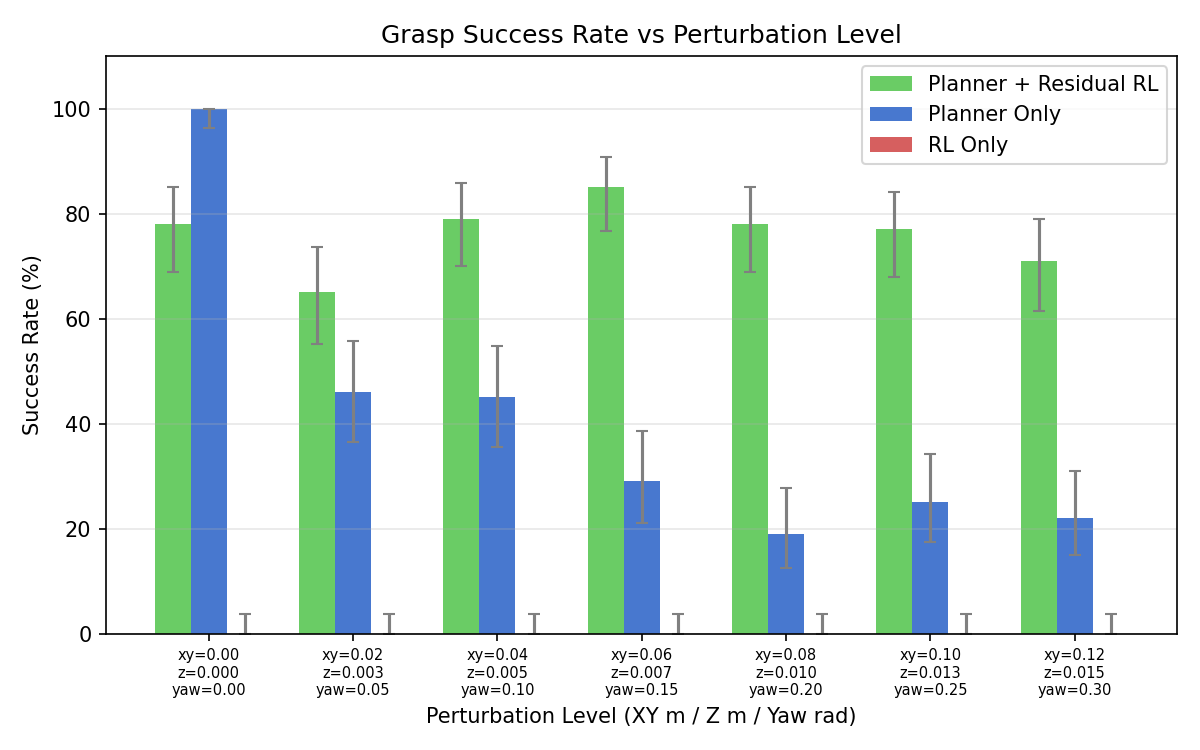
\includegraphics[width=\columnwidth]{figures/success_rate_vs_perturbation.png}
\caption{Grasp success rate versus planar cube perturbation, for the three evaluated methods. Error bars are Wilson $95\%$ intervals at $n = 100$. Hybrid (green) holds in $[0.65, 0.85]$ across every level; planner-only (blue) falls from $1.00$ to $0.22$; {\em rl\_only} (red) never succeeds. The gap between hybrid and planner-only exceeds $32$ percentage points from $\|\delta_{xy}\| \ge 0.04$ m onward, and peaks at $59$ points at $\|\delta_{xy}\| = 0.08$ m.}
\label{fig:success}
\end{figure}

\emph{Headline: Figure \ref{fig:success}.} The planner-only curve descends sharply at the first non-zero perturbation level and settles into a noisy plateau; the hybrid curve is essentially flat and above every planner point from $\|\delta_{xy}\| \ge 0.02$ m onward; the {\em rl\_only} curve is pinned at zero. The qualitative story is that the residual closes the planner's cliff almost entirely, and that by itself RL does not learn the task in our budget.

\begin{figure}[t]
\centering
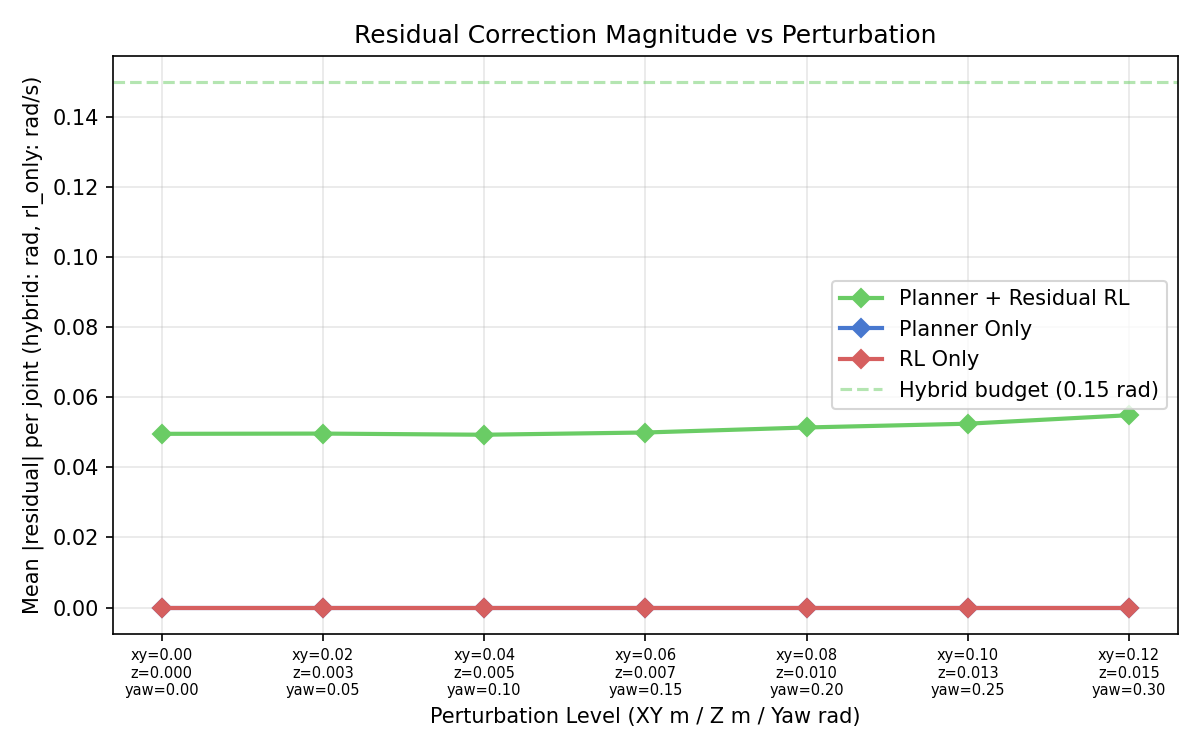
\includegraphics[width=\columnwidth]{figures/residual_magnitude.png}
\caption{Mean residual amplitude (rad) versus perturbation, across hybrid and {\em rl\_only}. Hybrid uses between $0.0496$ and $0.0549$ rad on average, which is roughly a third of the $0.15$ rad bound, and rises gently with $\delta$. The {\em rl\_only} curve is zero because in that mode the policy's action is applied as a full joint-velocity command rather than as a residual on top of a planner target, so the residual metric is not meaningfully defined.}
\label{fig:residual}
\end{figure}

\emph{The residual is load-bearing but not saturated.} Figure \ref{fig:residual} shows that mean residual amplitude in the hybrid runs lives between $0.0496$ rad at nominal and $0.0549$ rad at $\|\delta_{xy}\| = 0.12$ m. That is $33\%$--$37\%$ of the $0.15$ rad budget. The upward slope is gentle and monotone. Two things follow from this plot. First, the policy is actively using its budget---if it were not, we would expect mean residual to be near zero, and we see it well above that. Second, it is not slamming into the bound, which means the $\rho = 0.15$ rad cap is not itself the binding constraint on performance.

\begin{figure}[t]
\centering
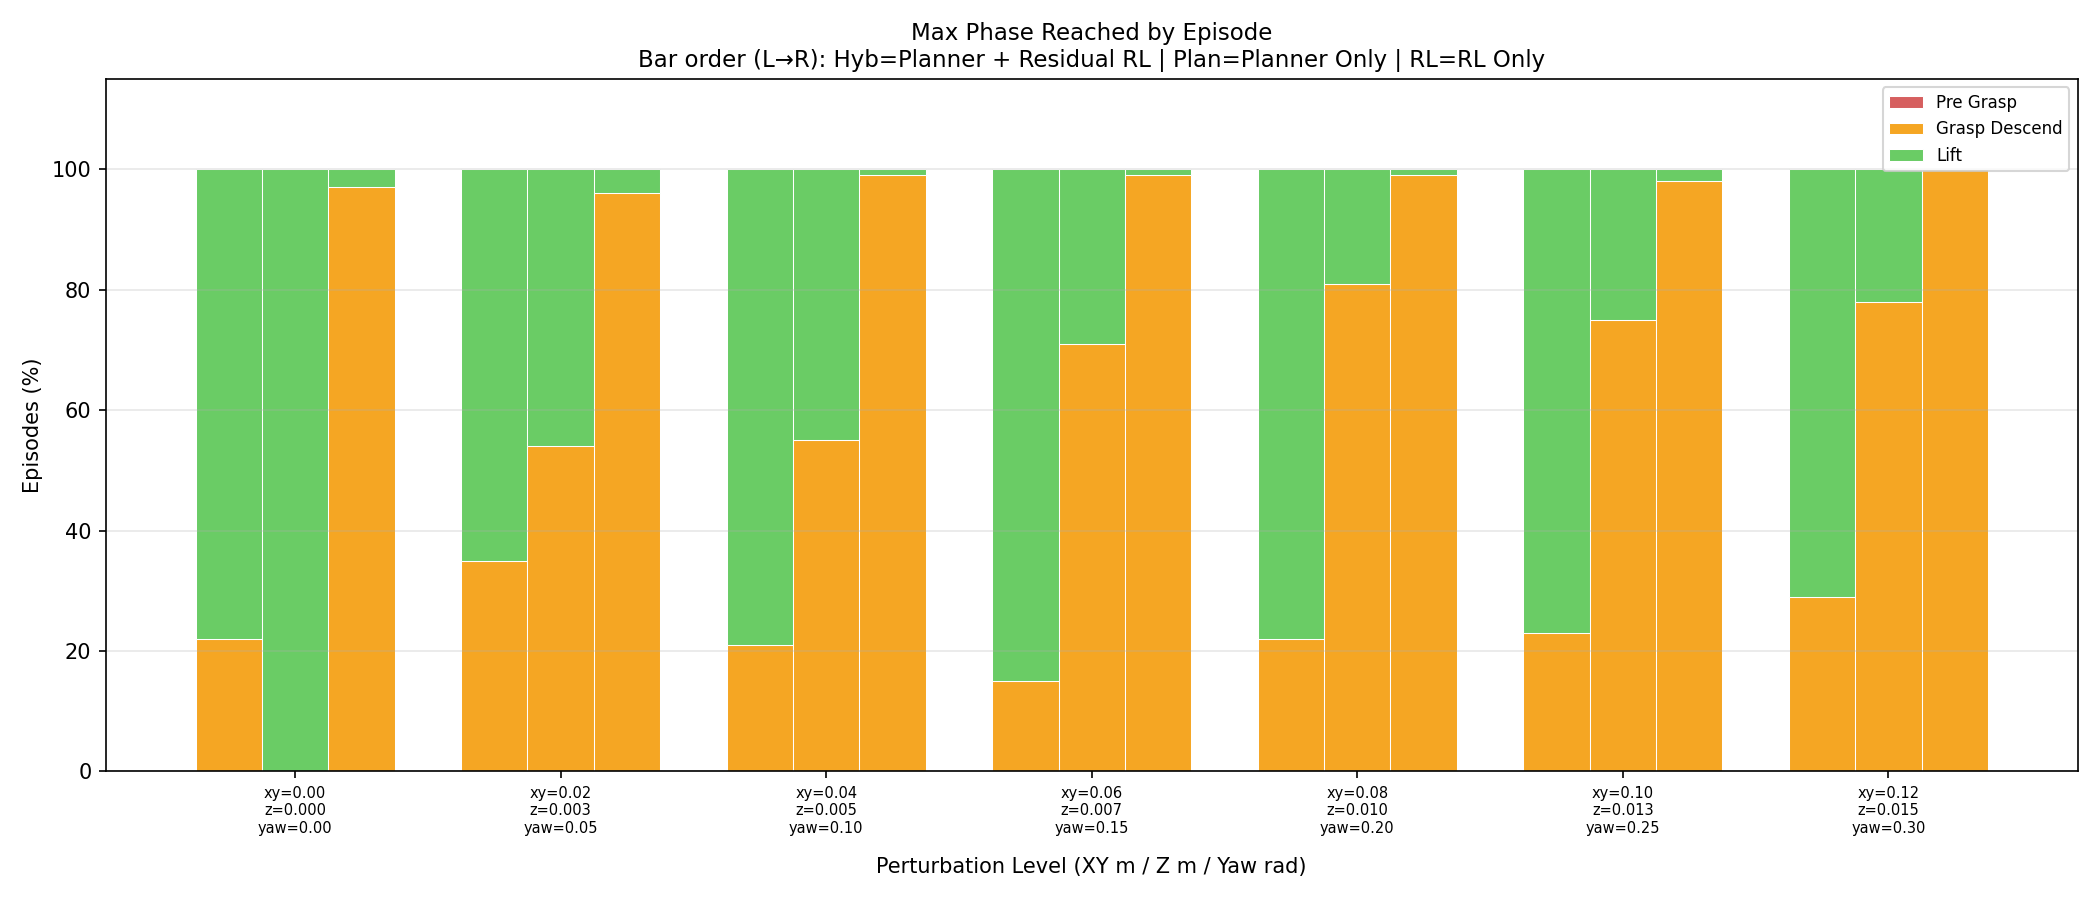
\includegraphics[width=\columnwidth]{figures/phase_breakdown.png}
\caption{Terminal-phase distribution by method, aggregated over all perturbation levels and episodes. Hybrid reaches LIFT in the large majority of episodes; planner-only reaches LIFT only when the cube happens to fall inside the jaw; {\em rl\_only} is effectively stuck in GRASP\_DESCEND ($\approx 97\%$ of episodes) and produces no lifts.}
\label{fig:phase}
\end{figure}

\emph{Ablation: Figure \ref{fig:phase}.} The {\em rl\_only} policy, with the classical scaffold removed, never learns to close a grasp. Aggregated over all $700$ {\em rl\_only} episodes in the eval, the terminal-phase breakdown is near-uniformly GRASP\_DESCEND (between $96\%$ and $100\%$ of episodes per level); the cube-lifted rate is zero across all seven perturbation magnitudes. Two numbers make the failure mode concrete. First, the end-effector-to-cube distance at termination, a proxy for ``did the arm actually arrive'', is flat at $0.096$--$0.121$ m across every perturbation level---it does not decrease when the cube is easier to reach. Second, the mean residual is zero because the action is interpreted as a full velocity command in this mode, not as a residual. The reading is that the policy learned an approximate joint-space trajectory from the shaped proximity reward, but never learned to close a Cartesian feedback loop on the cube. Without the PD+IK backbone, there was too much of the task left for the residual network to learn on the budget we gave it.

\emph{Hybrid at nominal is lower than planner at nominal.} This is the one result that is not flattering. At $\|\delta_{xy}\| = 0$, hybrid succeeds on $78$ of $100$ episodes while planner-only succeeds on $100$ of $100$. The simpler explanation is that the residual is always on during $\Phi_r$, and at zero perturbation the planner's waypoints are already correct, so the residual is mostly injecting noise. A confidence-gated residual that only activates when the policy has reason to believe the cube is displaced would plausibly fix this, and we flag it as a Milestone 3 candidate rather than a done deal.

\begin{figure}[t]
\centering
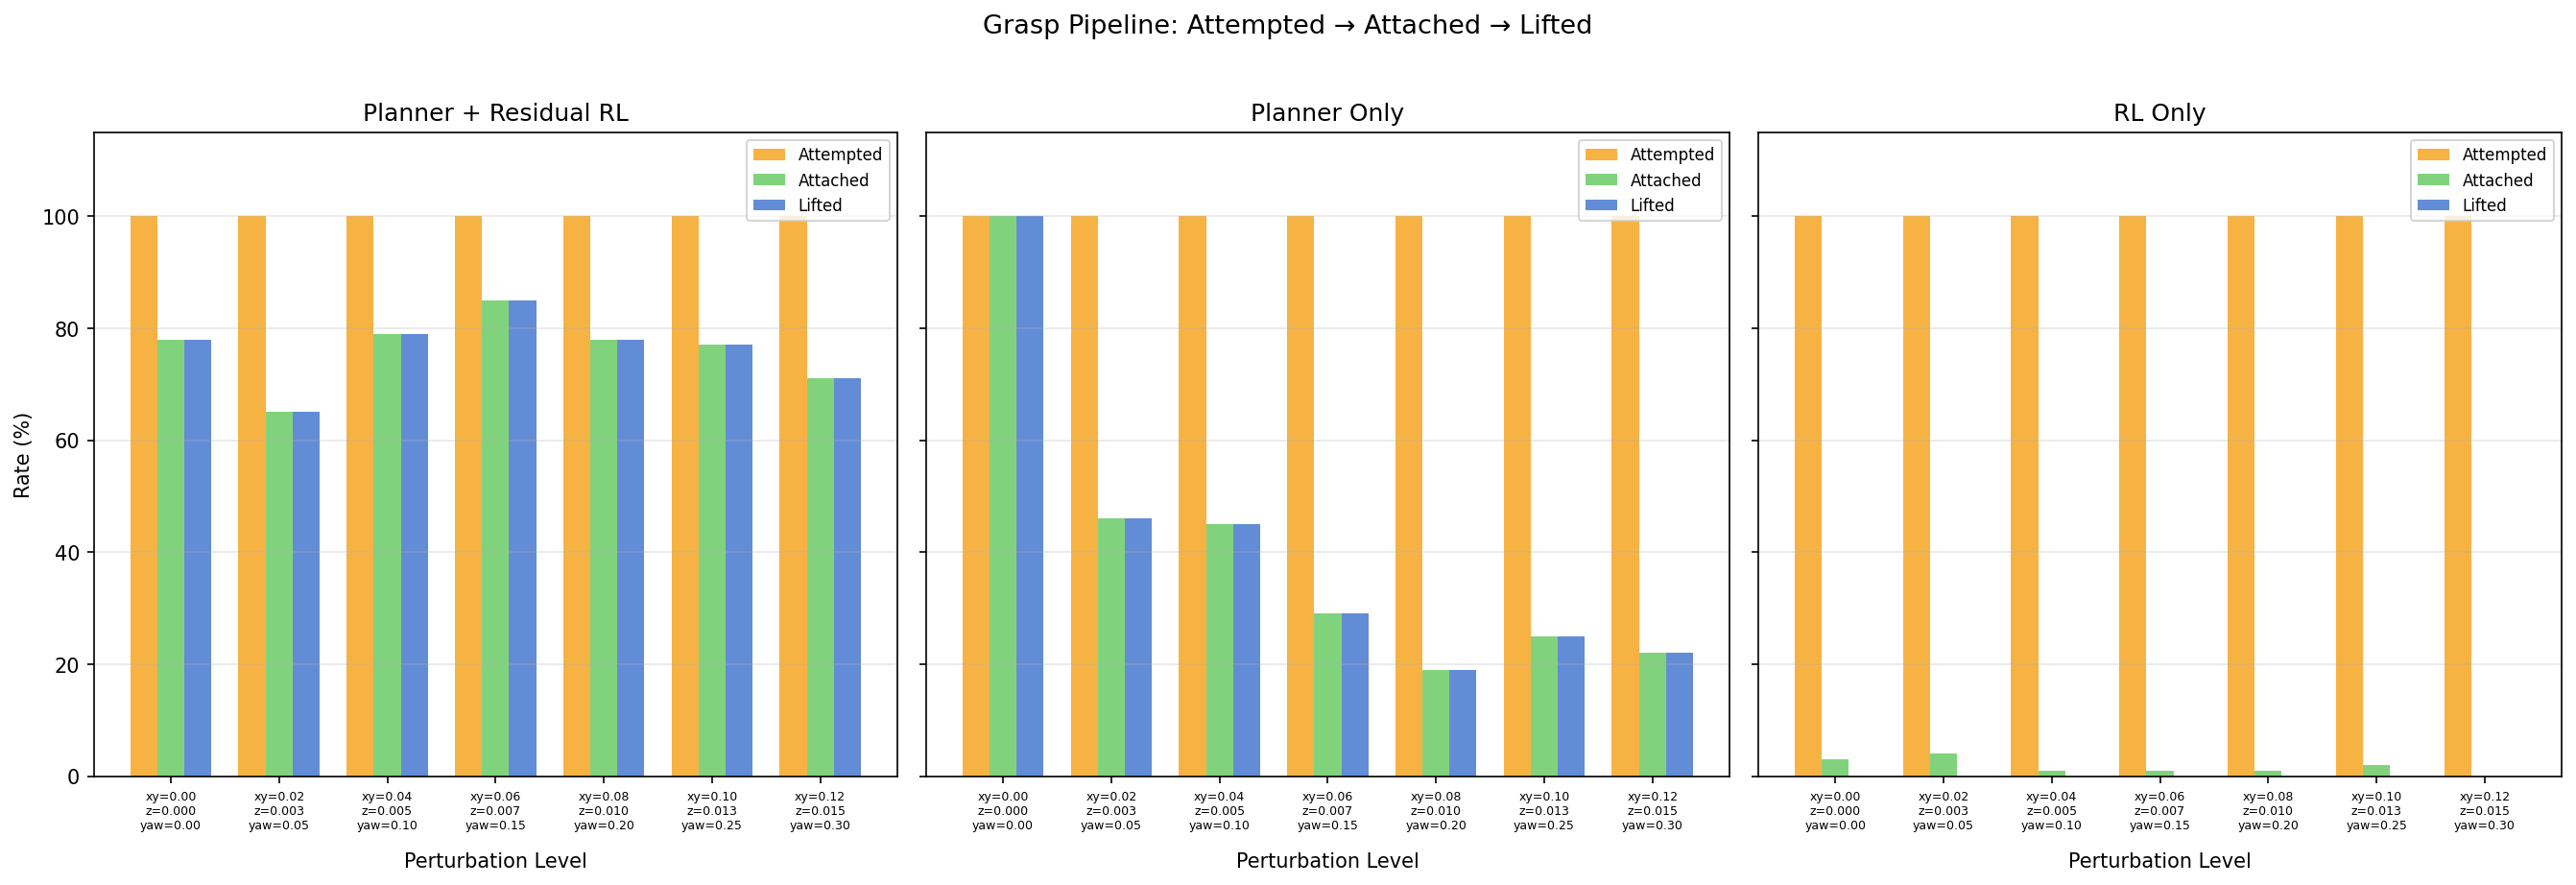
\includegraphics[width=\columnwidth]{figures/grasp_analysis.png}
\caption{Grasp-gate diagnostic: rate of grasp attempts, rate of successful attach, and cube-fall rate by method and perturbation. Hybrid attempts and attaches at the same rate. Planner-only attempts at every episode and attaches only in the successful subset. {\em rl\_only} attempts at every episode but essentially never attaches.}
\label{fig:grasp}
\end{figure}

Figure \ref{fig:grasp} offers one more piece of evidence for the load-bearing claim. The hybrid's attempt-rate and attach-rate track each other closely across perturbation, which is what a functioning grasp pipeline looks like. The planner's attempt-rate is uniform at one---the phase sequence always reaches GRASP\_CLOSE eventually---but its attach-rate drops with $\delta$, reflecting the cliff. The {\em rl\_only} curve shows an attempt-rate of one and an attach-rate near zero, which is the graphical form of ``looked roughly like a grasp, missed the cube''.

\begin{table}[t]
\centering
\caption{Success rate (and mean end-effector-to-cube distance, in meters) by method and planar perturbation magnitude. Numbers from {\tt results/m2/eval\_results.json}; each cell is $100$ episodes.}
\label{tab:summary}
\small
\begin{tabular}{c|cc|cc|cc}
\hline
$\|\delta_{xy}\|$ (m) & \multicolumn{2}{c|}{planner\_only} & \multicolumn{2}{c|}{hybrid} & \multicolumn{2}{c}{rl\_only}\\
  & $p$ & $d_{\mathrm{ee}}$ & $p$ & $d_{\mathrm{ee}}$ & $p$ & $d_{\mathrm{ee}}$\\
\hline
$0.00$ & $1.00$ & $0.020$ & $0.78$ & $0.022$ & $0.00$ & $0.112$\\
$0.02$ & $0.46$ & $0.022$ & $0.65$ & $0.021$ & $0.00$ & $0.096$\\
$0.04$ & $0.45$ & $0.027$ & $0.79$ & $0.020$ & $0.00$ & $0.097$\\
$0.06$ & $0.29$ & $0.037$ & $0.85$ & $0.018$ & $0.00$ & $0.098$\\
$0.08$ & $0.19$ & $0.045$ & $0.78$ & $0.023$ & $0.00$ & $0.099$\\
$0.10$ & $0.25$ & $0.053$ & $0.77$ & $0.023$ & $0.00$ & $0.098$\\
$0.12$ & $0.22$ & $0.056$ & $0.71$ & $0.026$ & $0.00$ & $0.121$\\
\hline
\end{tabular}
\end{table}

Table \ref{tab:summary} ties the pieces together. Two patterns are worth reading off. The planner's $d_{\mathrm{ee}}$ column grows almost linearly with $\|\delta_{xy}\|$, from $2.0$ cm at nominal to $5.6$ cm at the largest perturbation; the residual is directly canceling that drift. The hybrid's $d_{\mathrm{ee}}$ stays near two centimeters across the whole range, which is the quantitative form of ``the arm arrives at the real cube''. The {\em rl\_only} column is flat near ten centimeters and not dependent on perturbation, which is what a policy that has not learned to track looks like.

\section{CONCLUSION}
\label{sec:conclusion}

Residual reinforcement learning on top of a classical motion-planning backbone recovers most of the perturbation robustness that the backbone loses on its own, and it does so with a small learned correction that averages about a third of its allowed budget. The honest limitations are that the evaluation uses a single training seed, the grasp gate is still a geometric heuristic rather than a learned one, and the hybrid regresses at zero perturbation because the residual has no off-switch. A curriculum over perturbation magnitude, a multi-seed study, a learnable residual gate, and a sim-to-real preparation pass \cite{Tobin2017DomainRand} are the four extensions we would attempt next, in roughly that order. We also note without endorsement that an off-policy backbone such as SAC \cite{Haarnoja2018SAC} might recover some of the sample efficiency we lost to PPO's on-policy nature; it is not obvious this would change the conclusion.

\begin{thebibliography}{99}

\bibitem{Schulman2017PPO}
J. Schulman, F. Wolski, P. Dhariwal, A. Radford, and O. Klimov, ``Proximal policy optimization algorithms,'' \emph{arXiv:1707.06347}, 2017.

\bibitem{Johannink2019Residual}
T. Johannink, S. Bahl, A. Nair, J. Luo, A. Kumar, M. Loskyll, J. A. Ojea, E. Solowjow, and S. Levine, ``Residual reinforcement learning for robot control,'' in \emph{Proc. IEEE International Conference on Robotics and Automation (ICRA)}, 2019, pp. 6023--6029.

\bibitem{Silver2018Residual}
T. Silver, K. R. Allen, J. Tenenbaum, and L. P. Kaelbling, ``Residual policy learning,'' \emph{arXiv:1812.06298}, 2018.

\bibitem{Karaman2011RRTStar}
S. Karaman and E. Frazzoli, ``Sampling-based algorithms for optimal motion planning,'' \emph{The International Journal of Robotics Research}, vol. 30, no. 7, pp. 846--894, 2011.

\bibitem{Coumans2016PyBullet}
E. Coumans and Y. Bai, ``PyBullet, a Python module for physics simulation for games, robotics and machine learning,'' \url{http://pybullet.org}, 2016--2021.

\bibitem{Bou2023TorchRL}
A. Bou, M. Bettini, S. Dittert, V. Kumar, S. Sodhani, X. Yang, G. De Fabritiis, and V. Moens, ``TorchRL: A data-driven decision-making library for PyTorch,'' \emph{arXiv:2306.00577}, 2023.

\bibitem{Brown2001Wilson}
L. D. Brown, T. T. Cai, and A. DasGupta, ``Interval estimation for a binomial proportion,'' \emph{Statistical Science}, vol. 16, no. 2, pp. 101--133, 2001.

\bibitem{Tobin2017DomainRand}
J. Tobin, R. Fong, A. Ray, J. Schneider, W. Zaremba, and P. Abbeel, ``Domain randomization for transferring deep neural networks from simulation to the real world,'' in \emph{Proc. IEEE/RSJ International Conference on Intelligent Robots and Systems (IROS)}, 2017, pp. 23--30.

\bibitem{Haarnoja2018SAC}
T. Haarnoja, A. Zhou, P. Abbeel, and S. Levine, ``Soft actor-critic: Off-policy maximum entropy deep reinforcement learning with a stochastic actor,'' in \emph{Proc. International Conference on Machine Learning (ICML)}, 2018, pp. 1861--1870.

\bibitem{Levine2016Visuomotor}
S. Levine, C. Finn, T. Darrell, and P. Abbeel, ``End-to-end training of deep visuomotor policies,'' \emph{Journal of Machine Learning Research}, vol. 17, no. 39, pp. 1--40, 2016.

\bibitem{Haddadin2022Franka}
S. Haddadin, S. Parusel, L. Johannsmeier, S. Golz, S. Gabl, F. Walch, M. Sabaghian, C. J\"ahne, L. Hausperger, and S. Haddadin, ``The Franka Emika robot: A reference platform for robotics research and education,'' \emph{IEEE Robotics \& Automation Magazine}, vol. 29, no. 2, pp. 46--64, 2022.

\bibitem{Yu2020MetaWorld}
T. Yu, D. Quillen, Z. He, R. Julian, K. Hausman, C. Finn, and S. Levine, ``Meta-world: A benchmark and evaluation for multi-task and meta reinforcement learning,'' in \emph{Proc. Conference on Robot Learning (CoRL)}, 2020, pp. 1094--1100.

\end{thebibliography}

\end{document}
